% This is samplepaper.tex, a sample chapter demonstrating the
% LLNCS macro package for Springer Computer Science proceedings;
% Version 2.20 of 2017/10/04
%
\documentclass[runningheads]{llncs}
%
\usepackage{graphicx}
% Used for displaying a sample figure. If possible, figure files should
% be included in EPS format.
%
% If you use the hyperref package, please uncomment the following line
% to display URLs in blue roman font according to Springer's eBook style:
% \renewcommand\UrlFont{\color{blue}\rmfamily}

\begin{document}
%
\title{Issues in Benchmarks for Humanoid Robots\thanks{Supported by Ministry of Science and Technology (MOST), Taiwan, and National Taiwan Normal University (NTNU) Sprout Project)}}
%
%\titlerunning{Abbreviated paper title}
% If the paper title is too long for the running head, you can set
% an abbreviated paper title here
%
\author{Jacky Baltes\inst{1,2}\orcidID{0000-0003-3360-1892} 
\and
James Hsu\inst{1}\orcidID{0000-0002-3697-8401} 
\and
John Anderson\inst{2}
\and
Soroush Sadeghnejad\inst{3}
}
%
\authorrunning{J. Baltes et al.}
% First names are abbreviated in the running head.
% If there are more than two authors, 'et al.' is used.
%
\institute{National Taiwan Normal University (NTNU), Taipei, Taiwan 
\email{jacky.baltes@ntnu.edu.tw}\\
\url{https://sites.google.com/site/jackybaltes}
\and
University of Manitoba, Winnipeg, Canada
\and
Amirkabir University of Technology, Tehran, Iran
\email{s.sadeghnejad@aut.ac.ir}
}


%
\maketitle              % typeset the header of the contribution
%
\begin{abstract}
The paper describes the notion of the \emph{Don't Mess Up Period} as an important tool in evaluating the performance of humanoid and other robotic systems.
A simple model of a robotic system is developed and an investigation shows the impact of the various parameters on the DMUP is demonstrated and analyzed.
A comparison between the RoboCup Humanoid League Kid-Sized finals from 2009 and 2016 is used to estimate the improvements in the humanoid league during this time.

\keywords{Humanoid Robots  \and Benchmarks \and RoboCup.}
\end{abstract}
%
%
%
\section{Introduction}

Humanoid robotics is a active and popular research area and has led to many exciting new developments in areas such as robotics, computer vision, AI, machine learning, 
Three features of humanoid robots create unique challenges: bipedal locomotion and complex motion planning.

Just like other mobile robots, to be useful, a humanoid robot must be at the right place at the right time.
This means a humanoid robot must be able to walk, jog, or run in varying environments. 
In 2018, walking on flat surfaces has been demonstrated by many humanoid robots.
Humanoid robots are nowadays also able to walk up and down stairs.
However, uneven terrain, e.g., a hiking path, is still a difficult problem.
Researchers have also recently explored research in other forms of locomotion such as ice skating or skiing humanoid robots \cite{tu2017active}.
The problem of active balancing and push recovery is closely related to bi-pedal locomotion.
A humanoid robot must be able to tolerate bumps and pushes from other agents in the environment.

Another difference between humanoid robots and many other mobile robots is the fact that humanoid robots have many actuators and thus many degrees of freedom (DOF).
The large number of DOFs makes it possible to perform an almost infinite number of motions.
Humanoid robots are therefore able to dance and act more expressively than other robots.
The sheer size of the set of possible motions makes it difficult for a humanoid robot to create motion plans online, especially since the motions need to also obey kinematic and dynamic constraints so that the robot does not fall over during the action.
Note that in some domains, the ability to plan motions online is not necessary. 
For example, a soccer playing humanoid robot requires only about a dozen types of motions: walk forward, walk backward, turn left, turn right, shuffle left, shuffle right, kick left foot, kick right foot, stand up forward, stand up backward, dive left, dive right.
Some teams use omni-directional walking engines which combines the movement commands walk, turn, and sway into higher level motion primitives.
But in other domains, it is crucial to develop new motion online. 
For example, a spelunking robot intended to explore and save people lost in caves faces a limitless number of possible hand and foot hold combinations.
This makes it impossible to pre-program all necessary motions.
Humans are excellent at creating new motions, even in environments the question of the best motion seems to have been settled a long time ago.
For example, the front crawl in swimming, the Fosbury flop in high jump, and the V shape in ski jumping were introduced by individual athletes or small teams and have then dramatically changed the motions used in their respective sports.

Section~\ref{sec:dmup} introduces the notion of the Don't Mess Up Period (DMUP) as a measure for the intelligence of the robot.
Section~\ref{sec:conclusion} concludes the paper by comparing the average time difference between when the last set play and when a goal was scored in the RoboCup Humanoid Kid-Size league finals in 2009 and 2016.

\section{Don't Mess Up Period}
\label{sec:dmup}

However, the use of robot soccer as a benchmark problem for humanoid robots is problematic for another reason: It is difficult to show consistent progress.

Teams have developed ever more sophisticated hardware and software for robot soccer.
In particular, the areas of computer vision, walking and jogging, push recovery, localization (i.e., position of the robot on the playing field), and mapping (i.e., where are the other players on the field and where is the ball) have seen much development.

However, the general public, other researchers, and even people involved in the robot soccer community find it difficult to see what progress has been made in recent years.
A common metric for the progress that was used by trustees of RoboCup or the general public alike was the number of goals being scored in a match.
Even though goals are exciting and spectators want to see goals, the number of goals in a match does not demonstrate improvements in the research and is thus unsuitable as a benchmark for measuring the performance of robot soccer teams.

This problem is partially due to the fact that as the performance of the robots improves, the environment in which the robots play also changes.
For example, the RoboCup humanoid league has developed a road map to suggest a hoped for improvement in performance to achieve the 2050 goal of beating the human world champions in soccer.
This road map was created by the technical committee of the RoboCup humanoid league in collaboration with the team members of the RoboCup humanoid league.
The environment of the robot soccer competition have changed drastically in recent years,

\begin{enumerate}
\item The size of the playing field has increased, which means that: (a) the robots must move faster to cover the same percentage area of the field as previously, and (b) the vision must be more accurate to identify balls, goals, and field lines.

\item The playing surface was replaced by official FIFA certified AstroTurf. The AstroTurf is softer than the previous playing surface (carpet), and the robots must have more robust walking gaits than previously.

\item The ball has been replaced with standard FIFA soccer balls, which are much heavier than the previous tennis and plastic balls.

\item All color coded parts of the environment (e.g., red goal, yellow goal, orange ball) have been removed. 
The goals are now standard white goals and the soccer ball is a standard FIFA soccer ball (usually white or gray with some pattern).

\item The rules have been modified to more closely follow the FIFA rules.
For example, robots now must autonomously position themselves after stoppage in play and free kicks instead of time penalties are now used.

\item The focus of game play in the humanoid league has shifted from simply adding more players to drop-in games where robots must be able to play with robots programmed by other teams.

\end{enumerate}

This paper argues for the use of the Don't Mess Up Period (DMUP) as an important feature to track improvements in the skills and especially the robustness of the players.

The DMUP is defined as the amount of time that the robot must act intelligently before achieving a significant improvement to its current state.

For example, prior to 2007, a common strategy in the humanoid league was for the robot to:
\begin{enumerate}
    \item look for the orange ball,
    \item walk towards the ball,
    \item orbit around the ball until the ball is lined up with the opponents goal (either blue or yellow),
    \item and finally kick the ball towards that goal.
\end{enumerate}

Since the playing field was smooth and the ball light, robots were able to kick the ball at the goal fast enough so that it was difficult for the goal keeper robot to stop the ball before entering the goal.
This means that after acting intelligently for about 30 seconds (or after 300 decisions if we assume a 10Hz decision rate which is typical for humanoid robot participating in the humanoid league), the robot can achieve a major improvement to its state (a goal) and after a goal the state of the game will be reset to a known set play (kick off).

There were several games that showed extreme variants of this scenario. Team A scored a goal. Play continues with a kick-off for team B. 
If team B had problems walking to the ball at this time, then team A could score directly another goal after 10 seconds, because the rules disallowed goals from kick-offs for the team with the kick-off, but not the other team and the ball would be in play if not kicked for 10 seconds. 
Then team A scores again and the the cycle repeats itself.  
There were more high scoring games in the humanoid league at this time.

In 2017, the heavy ball, larger playing fields, and softer AstroTurf resulted in the fact that robots, especially in the kid-size where robots are less than 80cm tall, must now kick the ball three or four times before they can score a goal. The duration of this entire sequence is now close to 3 minutes before a robot can score a goal.

So the research in previous years has raised the DMUP from 30 secs. to 3 minutes or in other words, a factor of six. 
It shows that research progress in previous years has led to much more robust robots that can act autonomously for longer periods of time.

\section{Model and Analysis of Robustness and DMUP}
\label{sec:analysis}

In this section, we describe a high level model of a robot and investigate the impact of various factors on the DMUP for such a robot.

In this model, the performance of the robot is limited through two processes: standard ($S$) and mess-up ($E$) processes.

A robot senses its environment using several sensors (e.g., cameras, accelerometers, touch), combines its sensor readings and previous state into perceptions (e.g., ball in front), selects a goal (kick ball toward goal), develops a plan to achieve the goal (e.g., walk 10cm forward, then kick with left foot), and finally control the actuators to achieve the desired actions (e.g., move hip joint to 12 degrees). The actuators influence the environment, and the cycle repeats itself.
Note that this is a simple model of a robot. For example, a real robot may include several levels of abstractions between sensing and perception or several levels of abstractions in task or motion planning.

The state of the environment allows us to measure the performance of the robot at certain times.
To simplify the model, we assume that the robot is trying to achieve a performance score of 0.
However, not all states of the environment are feasible states from which the robot can autonomously continue.
Sometimes, the errors (i.e., divergence from 0) are so big that the robot cannot continue without human intervention (e.g., the robot looses its localization because it fails to detect field lines or goal posts).

In the model, the set of feasible states ranges from -1 to +1. 
Once the performance measure is outside of the feasible region, the robot must be reset.

Each step in this process (sensing, perception, task planning, motion planning, control) usually includes errors. 
Errors may be due to noise in the systems or unknowns in the reasoning process or faults in the hardware.

The performance of the robot depends on many random variables associated with the environment and processes in the robot itself.
Therefore, the performance of the robot depends on the sum of all these random variables.
Using the central limit theorem, we can expect that the performance of the robot is normally distributed.

Some of the errors in a robot are so catastrophic that they would immediately result in a state where human intervention is required (e.g., robot leaves playing field or robot is unable to stand up after a fall).
In our model, we assume that there is a constant critical error probability $e_{c}$ that will result in immediate failure of the robot.

Hence, our overall systems model $\mathcal{M}$ is described in equation~\ref{eq:model}.

\begin{equation}
    \label{eq:model}
    \mathcal{M} = 
       \left\{
          \begin{array}{cll}
            Critical & \mbox{with probability} &  e_c \\
            \sim \mathcal{N}(0, \sigma^2) & \mbox{with probability} & 1 - e_c \\
          \end{array}
       \right\}
\end{equation}

Figure~\ref{fig:pdf} shows a visualization of the resulting probability density function (pdf) of the model given various values for $e_c$ and $\sigma^2$.

One way to represent model $\mathcal{M}$ is via a standard deviation with variable cut-offs corresponding to the critical error regions. 
But in this paper, the pdf is shown ranging from -1.1 to +1.1.
The critical region is visualized as two extra regions, one from -1.1 to -1 and one from 1.0 to 1.1.
This representation gives a better indication of the relative size of the critical region versus the standard process as a range from $-\infty$ to $+\infty$.

\begin{figure}
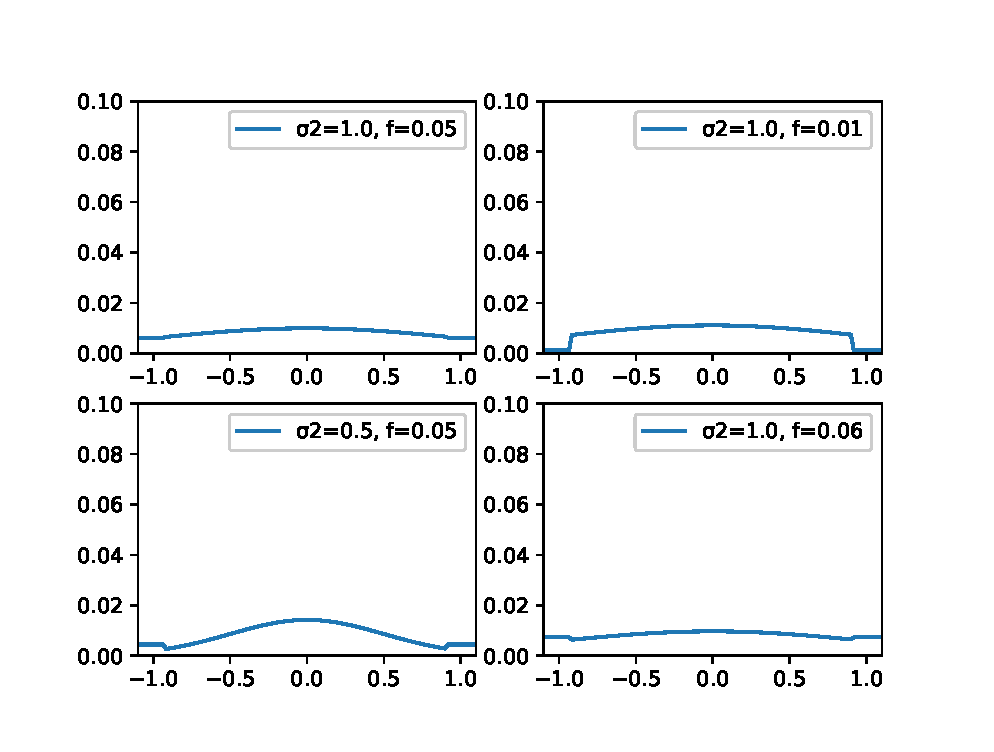
\includegraphics[width=\textwidth]{Figures/pdf2.eps}
\caption{The probability density function for the model $\mathcal{M}$ using different parameters for the crticial error rate $e_c$ and the variance of the standard process $\sigma^2$.} 
\label{fig:pdf}
\end{figure}

In our model, the performance of the robot is updated by drawing from $\mathcal{M}$ repeatedly until: (a) the performance has drifted outside of the range -1 to +1, or (b) until a critical error occurs, or (c) the maximum number of steps in the experiment have been reached.

\subsection{Performance Trace}

Figure {fig:plot} shows a trace of several experiments.
In some cases, the robot will complete the entire experiment successfully while performance remains in the allowed band (-1,+1). Termination of the experiment due to critical errors (red dashed line) and drifting errors (green dashed line).

\begin{figure}
\includegraphics[width=\textwidth]{Figures/plot2.eps}
\caption{Plot of the performance of our model. The solid line shows a robot that completes the entire experiment (50 steps), the green dashed line shows the performance drifting outside of the allowed region (-1 to +1) and the red dashed line shows a critical error.} 
\label{fig:plot}
\end{figure}

\subsection{DMUP}

Given the model $\mathcal{M}$, we can also investigate and analyse the

\begin{figure}
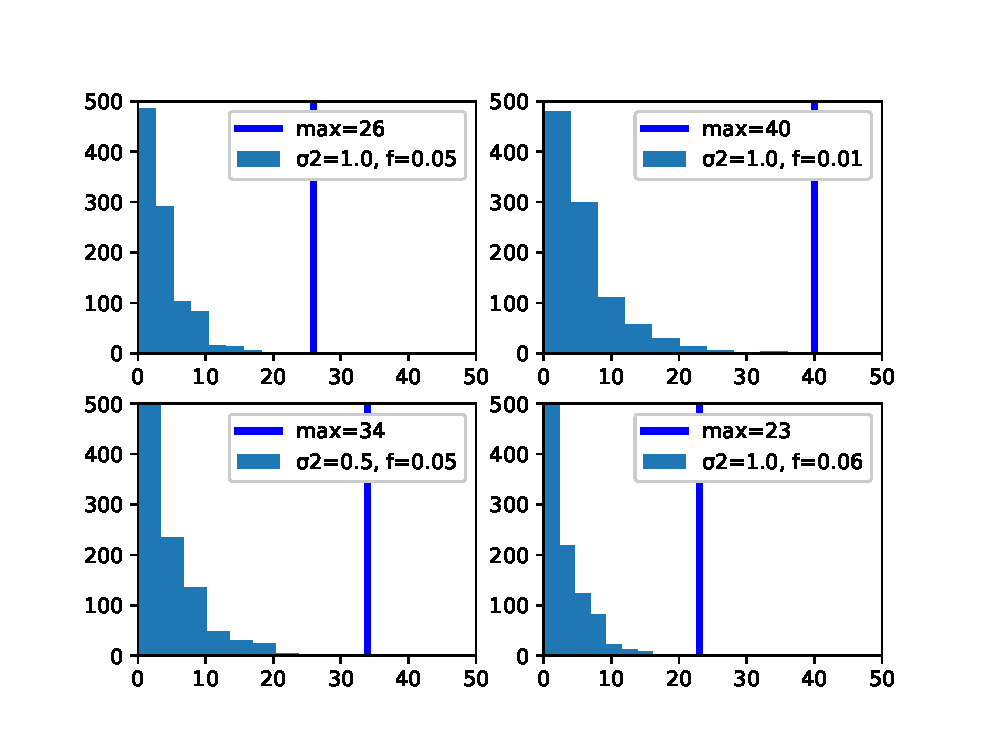
\includegraphics[width=\textwidth]{Figures/hist2.eps}
\caption{Plot of the performance of our model. The solid line shows a robot that completes the entire experiment (50 steps), the green dashed line shows the performance drifting outside of the allowed region (-1 to +1) and the red dashed line shows a critical error.} 
\label{fig:hist}
\end{figure}

\section{Conclusion}
\label{sec:conclusion}

We analyzed the final matches in RoboCup Humanoid League Kid-Size that were available on youtube in good quality without extensive cuts. The first match was the 2nd half of the 2009 Final between Darmstadt Dribblers and FUmanoids (https://www.youtube.com/watch?v=5wgyGglytKg).

The game was a high scoring match with many goals. 
The following table summarizes the duration between when a robot was in a set position and when a goal was scored (see Table~\ref{tab:2009kid}. 

\begin{table}[]
    \centering
    \caption{Goals Scored in the 2nd Half of the RoboCup Humanoid League Kid-Size Final 2009 between team Darmstadt Dribblers and FUmanoids}
    \label{tab:2009kid}
\begin{tabular}{|l|l|l|}
\hline 
Time Diff. & Game Time & Goal: Team and Position\\
\hline
1min 14s & 1:26 & Fumanoids; Near position\\	
30s	& 2:36 & Dribblers; Mid position\\	
28s	& 3:11 & Dribblers; Mid position\\	
3min 14s & 6:59	& Dribblers; Near position\\	
14s	& 7:53 & Dribblers; Mid position\\
41s	& 9:14 & Dribblers; Near position\\
\hline
\end{tabular}
\end{table}

In contrast, the time between a set play and when a goal was scored was significantly higher in the 2017 match between team Rhoban and team ZJUDancers.

%
% ---- Bibliography ----
%
% BibTeX users should specify bibliography style 'splncs04'.
% References will then be sorted and formatted in the correct style.
%
\bibliographystyle{splncs04}
\bibliography{benchmarking_humanoids}

\end{document}